

% Gradient Info
  
\tikzset {_az0w2hihs/.code = {\pgfsetadditionalshadetransform{ \pgftransformshift{\pgfpoint{0 bp } { 0 bp }  }  \pgftransformrotate{-270 }  \pgftransformscale{2 }  }}}
\pgfdeclarehorizontalshading{_kzikblmyk}{150bp}{rgb(0bp)=(1,1,1);
rgb(54.82142857142857bp)=(1,1,1);
rgb(62.5bp)=(0.61,0.61,0.61);
rgb(100bp)=(0.61,0.61,0.61)}

% Gradient Info
  
\tikzset {_ki58aoeq5/.code = {\pgfsetadditionalshadetransform{ \pgftransformshift{\pgfpoint{0 bp } { 0 bp }  }  \pgftransformrotate{-270 }  \pgftransformscale{2 }  }}}
\pgfdeclarehorizontalshading{_zqnhzoo5e}{150bp}{rgb(0bp)=(1,1,1);
rgb(54.82142857142857bp)=(1,1,1);
rgb(62.5bp)=(0.61,0.61,0.61);
rgb(100bp)=(0.61,0.61,0.61)}

% Gradient Info
  
\tikzset {_s2ca7cwt4/.code = {\pgfsetadditionalshadetransform{ \pgftransformshift{\pgfpoint{0 bp } { 0 bp }  }  \pgftransformrotate{-270 }  \pgftransformscale{2 }  }}}
\pgfdeclarehorizontalshading{_krjr92v7r}{150bp}{rgb(0bp)=(1,1,1);
rgb(54.82142857142857bp)=(1,1,1);
rgb(62.5bp)=(0.61,0.61,0.61);
rgb(100bp)=(0.61,0.61,0.61)}

% Gradient Info
  
\tikzset {_7zm702kfi/.code = {\pgfsetadditionalshadetransform{ \pgftransformshift{\pgfpoint{0 bp } { 0 bp }  }  \pgftransformrotate{0 }  \pgftransformscale{2 }  }}}
\pgfdeclarehorizontalshading{_sc2zfhq8p}{150bp}{rgb(0bp)=(0.29,0.56,0.89);
rgb(53.66071428571429bp)=(0.29,0.56,0.89);
rgb(62.5bp)=(0.82,0.01,0.11);
rgb(100bp)=(0.82,0.01,0.11)}

% Gradient Info
  
\tikzset {_947g3gh8b/.code = {\pgfsetadditionalshadetransform{ \pgftransformshift{\pgfpoint{0 bp } { -0.5 bp }  }  \pgftransformrotate{-90 }  \pgftransformscale{2 }  }}}
\pgfdeclarehorizontalshading{_mxat92h6q}{150bp}{rgb(0bp)=(1,1,1);
rgb(37.5bp)=(1,1,1);
rgb(62.5bp)=(0,0,0);
rgb(100bp)=(0,0,0)}
\tikzset{_zw40vxy9b/.code = {\pgfsetadditionalshadetransform{\pgftransformshift{\pgfpoint{0 bp } { -0.5 bp }  }  \pgftransformrotate{-90 }  \pgftransformscale{2 } }}}
\pgfdeclarehorizontalshading{_o3fnbd0uv} {150bp} {color(0bp)=(transparent!0);
color(37.5bp)=(transparent!0);
color(62.5bp)=(transparent!10);
color(100bp)=(transparent!10) } 
\pgfdeclarefading{_uc5rmmpr3}{\tikz \fill[shading=_o3fnbd0uv,_zw40vxy9b] (0,0) rectangle (50bp,50bp); } 

% Gradient Info
  
\tikzset {_oj9djzokq/.code = {\pgfsetadditionalshadetransform{ \pgftransformshift{\pgfpoint{0 bp } { 0 bp }  }  \pgftransformrotate{0 }  \pgftransformscale{2 }  }}}
\pgfdeclarehorizontalshading{_21zbm29sn}{150bp}{rgb(0bp)=(0.29,0.56,0.89);
rgb(52.85714285714286bp)=(0.29,0.56,0.89);
rgb(62.5bp)=(0.82,0.01,0.11);
rgb(100bp)=(0.82,0.01,0.11)}

% Gradient Info
  
\tikzset {_tvqijb5p1/.code = {\pgfsetadditionalshadetransform{ \pgftransformshift{\pgfpoint{0 bp } { -0.5 bp }  }  \pgftransformrotate{-90 }  \pgftransformscale{2 }  }}}
\pgfdeclarehorizontalshading{_8o8j9rz05}{150bp}{rgb(0bp)=(1,1,1);
rgb(37.5bp)=(1,1,1);
rgb(62.5bp)=(0,0,0);
rgb(100bp)=(0,0,0)}
\tikzset{_p06f5zkm0/.code = {\pgfsetadditionalshadetransform{\pgftransformshift{\pgfpoint{0 bp } { -0.5 bp }  }  \pgftransformrotate{-90 }  \pgftransformscale{2 } }}}
\pgfdeclarehorizontalshading{_wcrn90ura} {150bp} {color(0bp)=(transparent!0);
color(37.5bp)=(transparent!0);
color(62.5bp)=(transparent!10);
color(100bp)=(transparent!10) } 
\pgfdeclarefading{_y8qb6ci5m}{\tikz \fill[shading=_wcrn90ura,_p06f5zkm0] (0,0) rectangle (50bp,50bp); } 

% Gradient Info
  
\tikzset {_0coqb587w/.code = {\pgfsetadditionalshadetransform{ \pgftransformshift{\pgfpoint{0 bp } { 0 bp }  }  \pgftransformrotate{0 }  \pgftransformscale{2 }  }}}
\pgfdeclarehorizontalshading{_5rnivun9u}{150bp}{rgb(0bp)=(0.29,0.56,0.89);
rgb(56.51785714285714bp)=(0.29,0.56,0.89);
rgb(62.5bp)=(0.82,0.01,0.11);
rgb(100bp)=(0.82,0.01,0.11)}

% Gradient Info
  
\tikzset {_863t0pjv8/.code = {\pgfsetadditionalshadetransform{ \pgftransformshift{\pgfpoint{0 bp } { -0.5 bp }  }  \pgftransformrotate{-90 }  \pgftransformscale{2 }  }}}
\pgfdeclarehorizontalshading{_9vc02l939}{150bp}{rgb(0bp)=(1,1,1);
rgb(37.5bp)=(1,1,1);
rgb(62.5bp)=(0,0,0);
rgb(100bp)=(0,0,0)}
\tikzset{_db30gnpfg/.code = {\pgfsetadditionalshadetransform{\pgftransformshift{\pgfpoint{0 bp } { -0.5 bp }  }  \pgftransformrotate{-90 }  \pgftransformscale{2 } }}}
\pgfdeclarehorizontalshading{_np1wbih0r} {150bp} {color(0bp)=(transparent!0);
color(37.5bp)=(transparent!0);
color(62.5bp)=(transparent!10);
color(100bp)=(transparent!10) } 
\pgfdeclarefading{_0q079ch7h}{\tikz \fill[shading=_np1wbih0r,_db30gnpfg] (0,0) rectangle (50bp,50bp); } 
\tikzset{every picture/.style={line width=0.75pt}} %set default line width to 0.75pt        

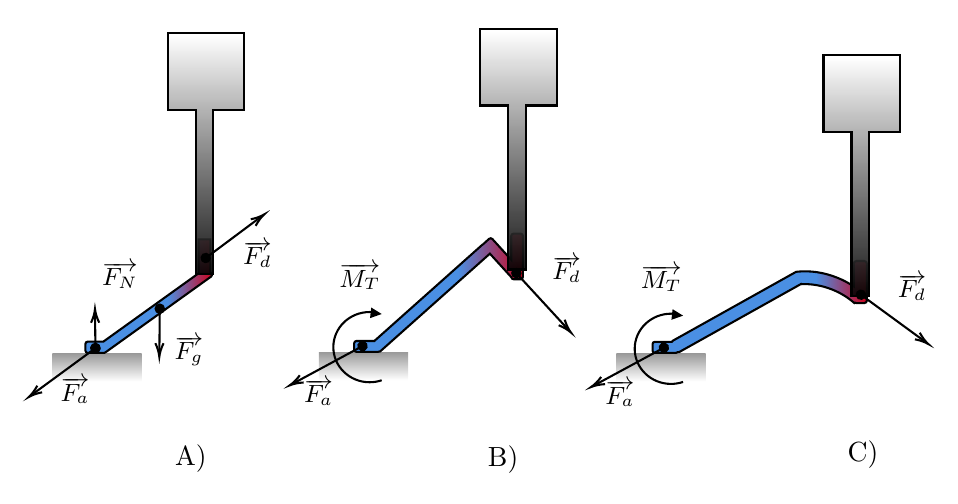
\begin{tikzpicture}[x=0.75pt,y=0.75pt,yscale=-1,xscale=1]
%uncomment if require: \path (0,300); %set diagram left start at 0, and has height of 300

%Shape: Square [id:dp8482883529416775] 
\draw  [draw opacity=0][shading=_kzikblmyk,_az0w2hihs] (366.67,189.33) -- (409.67,189.33) -- (409.67,232.33) -- (366.67,232.33) -- cycle ;
%Shape: Square [id:dp07525304880654671] 
\draw  [draw opacity=0][shading=_zqnhzoo5e,_ki58aoeq5] (223.33,188.67) -- (266.33,188.67) -- (266.33,231.67) -- (223.33,231.67) -- cycle ;
%Shape: Square [id:dp3833070704623305] 
\draw  [draw opacity=0][shading=_krjr92v7r,_s2ca7cwt4] (95,189.33) -- (138,189.33) -- (138,232.33) -- (95,232.33) -- cycle ;
%Shape: Path Data [id:dp1823169117970066] 
\path  [shading=_sc2zfhq8p,_7zm702kfi] (171.65,150.76) .. controls (171.95,151.2) and (171.85,151.8) .. (171.42,152.11) -- (120.9,188.35) .. controls (120.72,188.66) and (120.38,188.87) .. (119.99,188.87) -- (111.97,188.87) .. controls (111.38,188.87) and (110.9,188.38) .. (110.9,187.78) -- (110.9,184.52) .. controls (110.9,183.92) and (111.38,183.43) .. (111.97,183.43) -- (119.53,183.43) -- (165.44,150.49) -- (165.44,134.2) -- (171.13,134.2) -- (171.13,150.01) -- (171.65,150.76) -- cycle ; % for fading 
 \draw   (171.65,150.76) .. controls (171.95,151.2) and (171.85,151.8) .. (171.42,152.11) -- (120.9,188.35) .. controls (120.72,188.66) and (120.38,188.87) .. (119.99,188.87) -- (111.97,188.87) .. controls (111.38,188.87) and (110.9,188.38) .. (110.9,187.78) -- (110.9,184.52) .. controls (110.9,183.92) and (111.38,183.43) .. (111.97,183.43) -- (119.53,183.43) -- (165.44,150.49) -- (165.44,134.2) -- (171.13,134.2) -- (171.13,150.01) -- (171.65,150.76) -- cycle ; % for border 

%Shape: Path Data [id:dp7664852483691857] 
\path  [shading=_mxat92h6q,_947g3gh8b,path fading= _uc5rmmpr3 ,fading transform={xshift=2}] (172.5,150.75) -- (164,150.75) -- (164,71.75) -- (150.5,71.75) -- (150.5,34.75) -- (187.5,34.75) -- (187.5,71.75) -- (172.5,71.75) -- (172.5,150.75) -- cycle ; % for fading 
 \draw   (172.5,150.75) -- (164,150.75) -- (164,71.75) -- (150.5,71.75) -- (150.5,34.75) -- (187.5,34.75) -- (187.5,71.75) -- (172.5,71.75) -- (172.5,150.75) -- cycle ; % for border 

%Straight Lines [id:da8372784781387078] 
\draw    (168.86,143.14) -- (195.4,123.34) ;
\draw [shift={(197,122.14)}, rotate = 143.27] [color={rgb, 255:red, 0; green, 0; blue, 0 }  ][line width=0.75]    (6.56,-1.97) .. controls (4.17,-0.84) and (1.99,-0.18) .. (0,0) .. controls (1.99,0.18) and (4.17,0.84) .. (6.56,1.97)   ;
\draw [shift={(168.86,143.14)}, rotate = 323.27] [color={rgb, 255:red, 0; green, 0; blue, 0 }  ][fill={rgb, 255:red, 0; green, 0; blue, 0 }  ][line width=0.75]      (0, 0) circle [x radius= 2.01, y radius= 2.01]   ;
%Straight Lines [id:da5883622865301662] 
\draw    (115.71,186.57) -- (85.18,208.96) ;
\draw [shift={(83.57,210.14)}, rotate = 323.75] [color={rgb, 255:red, 0; green, 0; blue, 0 }  ][line width=0.75]    (6.56,-1.97) .. controls (4.17,-0.84) and (1.99,-0.18) .. (0,0) .. controls (1.99,0.18) and (4.17,0.84) .. (6.56,1.97)   ;
\draw [shift={(115.71,186.57)}, rotate = 143.75] [color={rgb, 255:red, 0; green, 0; blue, 0 }  ][fill={rgb, 255:red, 0; green, 0; blue, 0 }  ][line width=0.75]      (0, 0) circle [x radius= 2.01, y radius= 2.01]   ;
%Straight Lines [id:da9559015453503384] 
\draw    (115.71,186.57) -- (115.52,169.75) ;
\draw [shift={(115.5,167.75)}, rotate = 89.35] [color={rgb, 255:red, 0; green, 0; blue, 0 }  ][line width=0.75]    (6.56,-1.97) .. controls (4.17,-0.84) and (1.99,-0.18) .. (0,0) .. controls (1.99,0.18) and (4.17,0.84) .. (6.56,1.97)   ;
\draw [shift={(115.71,186.57)}, rotate = 269.35] [color={rgb, 255:red, 0; green, 0; blue, 0 }  ][fill={rgb, 255:red, 0; green, 0; blue, 0 }  ][line width=0.75]      (0, 0) circle [x radius= 2.01, y radius= 2.01]   ;
%Straight Lines [id:da8008989184780188] 
\draw    (146.71,167.57) -- (146.52,188.75) ;
\draw [shift={(146.5,190.75)}, rotate = 270.53] [color={rgb, 255:red, 0; green, 0; blue, 0 }  ][line width=0.75]    (6.56,-1.97) .. controls (4.17,-0.84) and (1.99,-0.18) .. (0,0) .. controls (1.99,0.18) and (4.17,0.84) .. (6.56,1.97)   ;
\draw [shift={(146.71,167.57)}, rotate = 90.53] [color={rgb, 255:red, 0; green, 0; blue, 0 }  ][fill={rgb, 255:red, 0; green, 0; blue, 0 }  ][line width=0.75]      (0, 0) circle [x radius= 2.01, y radius= 2.01]   ;
%Shape: Path Data [id:dp9292649336162639] 
\path  [shading=_21zbm29sn,_oj9djzokq] (241.44,183.13) -- (250.08,183.13) -- (302.2,136.68) .. controls (302.34,136.56) and (302.5,136.48) .. (302.66,136.43) .. controls (302.72,136.34) and (302.79,136.26) .. (302.87,136.18) -- (305.37,133.91) .. controls (305.83,133.49) and (306.54,133.53) .. (306.96,133.99) -- (316.05,143.99) -- (316.05,132.53) .. controls (316.05,131.9) and (316.56,131.4) .. (317.18,131.4) -- (320.55,131.4) .. controls (321.18,131.4) and (321.68,131.9) .. (321.68,132.53) -- (321.68,152.23) .. controls (321.68,152.85) and (321.18,153.36) .. (320.55,153.36) -- (317.18,153.36) .. controls (316.6,153.36) and (316.12,152.92) .. (316.06,152.36) .. controls (316.06,152.36) and (316.05,152.36) .. (316.05,152.35) -- (305.77,141.04) -- (252.9,188.15) .. controls (252.57,188.45) and (252.11,188.51) .. (251.73,188.36) .. controls (251.72,188.36) and (251.71,188.36) .. (251.7,188.36) -- (241.44,188.36) .. controls (240.86,188.36) and (240.39,187.89) .. (240.39,187.31) -- (240.39,184.17) .. controls (240.39,183.59) and (240.86,183.13) .. (241.44,183.13) -- cycle ; % for fading 
 \draw   (241.44,183.13) -- (250.08,183.13) -- (302.2,136.68) .. controls (302.34,136.56) and (302.5,136.48) .. (302.66,136.43) .. controls (302.72,136.34) and (302.79,136.26) .. (302.87,136.18) -- (305.37,133.91) .. controls (305.83,133.49) and (306.54,133.53) .. (306.96,133.99) -- (316.05,143.99) -- (316.05,132.53) .. controls (316.05,131.9) and (316.56,131.4) .. (317.18,131.4) -- (320.55,131.4) .. controls (321.18,131.4) and (321.68,131.9) .. (321.68,132.53) -- (321.68,152.23) .. controls (321.68,152.85) and (321.18,153.36) .. (320.55,153.36) -- (317.18,153.36) .. controls (316.6,153.36) and (316.12,152.92) .. (316.06,152.36) .. controls (316.06,152.36) and (316.05,152.36) .. (316.05,152.35) -- (305.77,141.04) -- (252.9,188.15) .. controls (252.57,188.45) and (252.11,188.51) .. (251.73,188.36) .. controls (251.72,188.36) and (251.71,188.36) .. (251.7,188.36) -- (241.44,188.36) .. controls (240.86,188.36) and (240.39,187.89) .. (240.39,187.31) -- (240.39,184.17) .. controls (240.39,183.59) and (240.86,183.13) .. (241.44,183.13) -- cycle ; % for border 

%Shape: Path Data [id:dp640912868425004] 
\path  [shading=_8o8j9rz05,_tvqijb5p1,path fading= _y8qb6ci5m ,fading transform={xshift=2}] (323.2,148.67) -- (314.7,148.67) -- (314.7,69.67) -- (301.2,69.67) -- (301.2,32.67) -- (338.2,32.67) -- (338.2,69.67) -- (323.2,69.67) -- (323.2,148.67) -- cycle ; % for fading 
 \draw   (323.2,148.67) -- (314.7,148.67) -- (314.7,69.67) -- (301.2,69.67) -- (301.2,32.67) -- (338.2,32.67) -- (338.2,69.67) -- (323.2,69.67) -- (323.2,148.67) -- cycle ; % for border 

%Straight Lines [id:da4735344307781033] 
\draw    (244.38,185.57) -- (227.51,194.68) -- (211.09,203.55) ;
\draw [shift={(209.33,204.5)}, rotate = 331.63] [color={rgb, 255:red, 0; green, 0; blue, 0 }  ][line width=0.75]    (6.56,-1.97) .. controls (4.17,-0.84) and (1.99,-0.18) .. (0,0) .. controls (1.99,0.18) and (4.17,0.84) .. (6.56,1.97)   ;
\draw [shift={(244.38,185.57)}, rotate = 151.63] [color={rgb, 255:red, 0; green, 0; blue, 0 }  ][fill={rgb, 255:red, 0; green, 0; blue, 0 }  ][line width=0.75]      (0, 0) circle [x radius= 2.01, y radius= 2.01]   ;
%Straight Lines [id:da8646577096120663] 
\draw    (318.51,150.44) -- (327.68,160.41) -- (343.45,177.56) ;
\draw [shift={(344.8,179.03)}, rotate = 227.41] [color={rgb, 255:red, 0; green, 0; blue, 0 }  ][line width=0.75]    (6.56,-1.97) .. controls (4.17,-0.84) and (1.99,-0.18) .. (0,0) .. controls (1.99,0.18) and (4.17,0.84) .. (6.56,1.97)   ;
\draw [shift={(318.51,150.44)}, rotate = 47.41] [color={rgb, 255:red, 0; green, 0; blue, 0 }  ][fill={rgb, 255:red, 0; green, 0; blue, 0 }  ][line width=0.75]      (0, 0) circle [x radius= 2.01, y radius= 2.01]   ;
%Shape: Arc [id:dp05193043475644299] 
\draw  [draw opacity=0] (253.64,202.05) .. controls (251.83,202.66) and (249.87,203) .. (247.83,203) .. controls (238.17,203) and (230.33,195.43) .. (230.33,186.08) .. controls (230.33,176.74) and (238.17,169.17) .. (247.83,169.17) .. controls (249.87,169.17) and (251.83,169.5) .. (253.64,170.12) -- (247.83,186.08) -- cycle ; \draw    (253.64,202.05) .. controls (251.83,202.66) and (249.87,203) .. (247.83,203) .. controls (238.17,203) and (230.33,195.43) .. (230.33,186.08) .. controls (230.33,176.74) and (238.17,169.17) .. (247.83,169.17) .. controls (248.83,169.17) and (249.81,169.25) .. (250.76,169.4) ; \draw [shift={(253.64,170.12)}, rotate = 186.14] [fill={rgb, 255:red, 0; green, 0; blue, 0 }  ][line width=0.08]  [draw opacity=0] (5.36,-2.57) -- (0,0) -- (5.36,2.57) -- cycle    ; 
%Shape: Path Data [id:dp083988650529362] 
\path  [shading=_5rnivun9u,_0coqb587w] (385.22,183.51) -- (393.45,183.51) .. controls (393.56,183.28) and (393.74,183.09) .. (393.97,182.95) -- (453.28,149.81) .. controls (453.59,149.63) and (453.95,149.6) .. (454.26,149.7) .. controls (460.2,149.16) and (466.69,150.06) .. (473.03,152.6) .. controls (475.95,153.76) and (478.64,155.2) .. (481.08,156.84) -- (481.08,145.87) .. controls (481.08,145.17) and (481.65,144.6) .. (482.35,144.6) -- (486.15,144.6) .. controls (486.85,144.6) and (487.42,145.17) .. (487.42,145.87) -- (487.42,163.6) .. controls (487.42,164.3) and (486.85,164.86) .. (486.15,164.86) -- (482.35,164.86) .. controls (482.1,164.86) and (481.86,164.79) .. (481.66,164.66) -- (481.35,164.86) .. controls (478.42,162.25) and (474.83,160) .. (470.73,158.36) .. controls (465.56,156.29) and (460.31,155.48) .. (455.53,155.78) -- (455.52,155.74) -- (397.03,188.43) .. controls (396.74,188.59) and (396.42,188.62) .. (396.12,188.55) .. controls (395.93,188.76) and (395.65,188.89) .. (395.34,188.89) -- (385.22,188.89) .. controls (384.63,188.89) and (384.15,188.4) .. (384.15,187.81) -- (384.15,184.58) .. controls (384.15,183.99) and (384.63,183.51) .. (385.22,183.51) -- cycle ; % for fading 
 \draw   (385.22,183.51) -- (393.45,183.51) .. controls (393.56,183.28) and (393.74,183.09) .. (393.97,182.95) -- (453.28,149.81) .. controls (453.59,149.63) and (453.95,149.6) .. (454.26,149.7) .. controls (460.2,149.16) and (466.69,150.06) .. (473.03,152.6) .. controls (475.95,153.76) and (478.64,155.2) .. (481.08,156.84) -- (481.08,145.87) .. controls (481.08,145.17) and (481.65,144.6) .. (482.35,144.6) -- (486.15,144.6) .. controls (486.85,144.6) and (487.42,145.17) .. (487.42,145.87) -- (487.42,163.6) .. controls (487.42,164.3) and (486.85,164.86) .. (486.15,164.86) -- (482.35,164.86) .. controls (482.1,164.86) and (481.86,164.79) .. (481.66,164.66) -- (481.35,164.86) .. controls (478.42,162.25) and (474.83,160) .. (470.73,158.36) .. controls (465.56,156.29) and (460.31,155.48) .. (455.53,155.78) -- (455.52,155.74) -- (397.03,188.43) .. controls (396.74,188.59) and (396.42,188.62) .. (396.12,188.55) .. controls (395.93,188.76) and (395.65,188.89) .. (395.34,188.89) -- (385.22,188.89) .. controls (384.63,188.89) and (384.15,188.4) .. (384.15,187.81) -- (384.15,184.58) .. controls (384.15,183.99) and (384.63,183.51) .. (385.22,183.51) -- cycle ; % for border 

%Shape: Path Data [id:dp4888310079490593] 
\path  [shading=_9vc02l939,_863t0pjv8,path fading= _0q079ch7h ,fading transform={xshift=2}] (488.5,161.47) -- (480,161.47) -- (480,82.47) -- (466.5,82.47) -- (466.5,45.47) -- (503.5,45.47) -- (503.5,82.47) -- (488.5,82.47) -- (488.5,161.47) -- cycle ; % for fading 
 \draw   (488.5,161.47) -- (480,161.47) -- (480,82.47) -- (466.5,82.47) -- (466.5,45.47) -- (503.5,45.47) -- (503.5,82.47) -- (488.5,82.47) -- (488.5,161.47) -- cycle ; % for border 

%Straight Lines [id:da7299773302791036] 
\draw    (389.58,186.37) -- (372.71,195.48) -- (356.29,204.35) ;
\draw [shift={(354.53,205.3)}, rotate = 331.63] [color={rgb, 255:red, 0; green, 0; blue, 0 }  ][line width=0.75]    (6.56,-1.97) .. controls (4.17,-0.84) and (1.99,-0.18) .. (0,0) .. controls (1.99,0.18) and (4.17,0.84) .. (6.56,1.97)   ;
\draw [shift={(389.58,186.37)}, rotate = 151.63] [color={rgb, 255:red, 0; green, 0; blue, 0 }  ][fill={rgb, 255:red, 0; green, 0; blue, 0 }  ][line width=0.75]      (0, 0) circle [x radius= 2.01, y radius= 2.01]   ;
%Shape: Arc [id:dp5816487923294394] 
\draw  [draw opacity=0] (398.84,202.85) .. controls (397.03,203.46) and (395.07,203.8) .. (393.03,203.8) .. controls (383.37,203.8) and (375.53,196.23) .. (375.53,186.88) .. controls (375.53,177.54) and (383.37,169.97) .. (393.03,169.97) .. controls (395.07,169.97) and (397.03,170.3) .. (398.84,170.92) -- (393.03,186.88) -- cycle ; \draw    (398.84,202.85) .. controls (397.03,203.46) and (395.07,203.8) .. (393.03,203.8) .. controls (383.37,203.8) and (375.53,196.23) .. (375.53,186.88) .. controls (375.53,177.54) and (383.37,169.97) .. (393.03,169.97) .. controls (394.03,169.97) and (395.01,170.05) .. (395.96,170.2) ; \draw [shift={(398.84,170.92)}, rotate = 186.14] [fill={rgb, 255:red, 0; green, 0; blue, 0 }  ][line width=0.08]  [draw opacity=0] (5.36,-2.57) -- (0,0) -- (5.36,2.57) -- cycle    ; 
%Straight Lines [id:da3777206426102483] 
\draw    (484.51,160.84) -- (515.39,183.42) ;
\draw [shift={(517,184.6)}, rotate = 216.18] [color={rgb, 255:red, 0; green, 0; blue, 0 }  ][line width=0.75]    (6.56,-1.97) .. controls (4.17,-0.84) and (1.99,-0.18) .. (0,0) .. controls (1.99,0.18) and (4.17,0.84) .. (6.56,1.97)   ;
\draw [shift={(484.51,160.84)}, rotate = 36.18] [color={rgb, 255:red, 0; green, 0; blue, 0 }  ][fill={rgb, 255:red, 0; green, 0; blue, 0 }  ][line width=0.75]      (0, 0) circle [x radius= 2.01, y radius= 2.01]   ;

% Text Node
\draw (185.43,133.57) node [anchor=north west][inner sep=0.75pt]  [font=\small] [align=left] {$\displaystyle \overrightarrow{F_{d}}$};
% Text Node
\draw (97.43,199.29) node [anchor=north west][inner sep=0.75pt]  [font=\small] [align=left] {$\displaystyle \overrightarrow{F_{a}}$};
% Text Node
\draw (117.43,143.79) node [anchor=north west][inner sep=0.75pt]  [font=\small] [align=left] {$\displaystyle \overrightarrow{F_{N}}$};
% Text Node
\draw (152.43,179.29) node [anchor=north west][inner sep=0.75pt]  [font=\small] [align=left] {$\displaystyle \overrightarrow{F_{g}}$};
% Text Node
\draw (214.76,199.95) node [anchor=north west][inner sep=0.75pt]  [font=\small] [align=left] {$\displaystyle \overrightarrow{F_{a}}$};
% Text Node
\draw (334.43,140.57) node [anchor=north west][inner sep=0.75pt]  [font=\small] [align=left] {$\displaystyle \overrightarrow{F_{d}}$};
% Text Node
\draw (231.76,144.29) node [anchor=north west][inner sep=0.75pt]  [font=\small] [align=left] {$\displaystyle \overrightarrow{M_{T}}$};
% Text Node
\draw (359.96,200.75) node [anchor=north west][inner sep=0.75pt]  [font=\small] [align=left] {$\displaystyle \overrightarrow{F_{a}}$};
% Text Node
\draw (376.96,145.09) node [anchor=north west][inner sep=0.75pt]  [font=\small] [align=left] {$\displaystyle \overrightarrow{M_{T}}$};
% Text Node
\draw (500.83,149.37) node [anchor=north west][inner sep=0.75pt]  [font=\small] [align=left] {$\displaystyle \overrightarrow{F_{d}}$};
% Text Node
\draw (152.67,231.67) node [anchor=north west][inner sep=0.75pt]   [align=left] {A)};
% Text Node
\draw (303.33,232.33) node [anchor=north west][inner sep=0.75pt]   [align=left] {B)};
% Text Node
\draw (476.67,229.67) node [anchor=north west][inner sep=0.75pt]   [align=left] {C)};


\end{tikzpicture}
